\documentclass{minimal}
\usepackage{graphicx,color}
\usepackage[utf8]{inputenc}
\usepackage[papersize={335.00bp,251.00bp},text={335.00bp,251.00bp}]{geometry}
\begin{document}
\centering
% Title: Figure 1
% Creator: GL2PS 1.4.2, (C) 1999-2020 C. Geuzaine
% For: Octave
% CreationDate: Tue Dec 13 23:14:10 2022
\setlength{\unitlength}{1pt}
\begin{picture}(0,0)
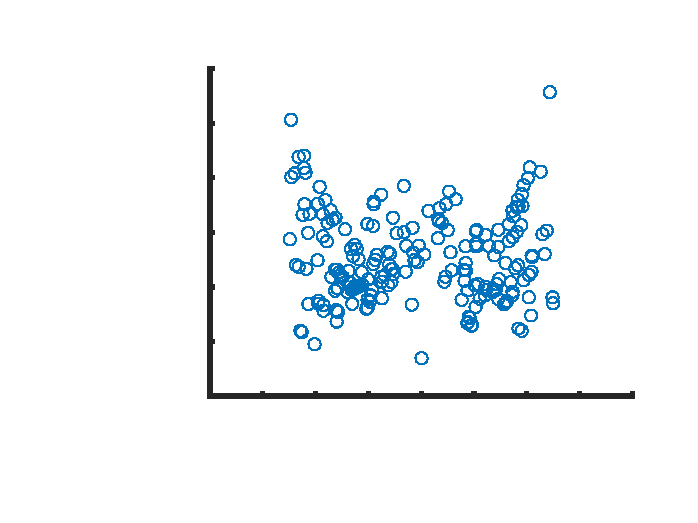
\includegraphics[scale=1]{DoubleKapitzaPoincareMapped-inc}
\end{picture}%
\begin{picture}(335,251)(0,0)
\fontsize{22}{0}\selectfont\put(100.789,44.4581){\makebox(0,0)[t]{\textcolor[rgb]{0.15,0.15,0.15}{{-0.8}}}}
\fontsize{22}{0}\selectfont\put(126.132,44.4581){\makebox(0,0)[t]{\textcolor[rgb]{0.15,0.15,0.15}{{-0.6}}}}
\fontsize{22}{0}\selectfont\put(151.475,44.4581){\makebox(0,0)[t]{\textcolor[rgb]{0.15,0.15,0.15}{{-0.4}}}}
\fontsize{22}{0}\selectfont\put(176.817,44.4581){\makebox(0,0)[t]{\textcolor[rgb]{0.15,0.15,0.15}{{-0.2}}}}
\fontsize{22}{0}\selectfont\put(202.16,44.4581){\makebox(0,0)[t]{\textcolor[rgb]{0.15,0.15,0.15}{{0}}}}
\fontsize{22}{0}\selectfont\put(227.503,44.4581){\makebox(0,0)[t]{\textcolor[rgb]{0.15,0.15,0.15}{{0.2}}}}
\fontsize{22}{0}\selectfont\put(252.846,44.4581){\makebox(0,0)[t]{\textcolor[rgb]{0.15,0.15,0.15}{{0.4}}}}
\fontsize{22}{0}\selectfont\put(278.188,44.4581){\makebox(0,0)[t]{\textcolor[rgb]{0.15,0.15,0.15}{{0.6}}}}
\fontsize{22}{0}\selectfont\put(303.531,44.4581){\makebox(0,0)[t]{\textcolor[rgb]{0.15,0.15,0.15}{{0.8}}}}
\fontsize{22}{0}\selectfont\put(89.8033,60.9621){\makebox(0,0)[r]{\textcolor[rgb]{0.15,0.15,0.15}{{-10}}}}
\fontsize{22}{0}\selectfont\put(89.8033,87.1351){\makebox(0,0)[r]{\textcolor[rgb]{0.15,0.15,0.15}{{0}}}}
\fontsize{22}{0}\selectfont\put(89.8033,113.308){\makebox(0,0)[r]{\textcolor[rgb]{0.15,0.15,0.15}{{10}}}}
\fontsize{22}{0}\selectfont\put(89.8033,139.481){\makebox(0,0)[r]{\textcolor[rgb]{0.15,0.15,0.15}{{20}}}}
\fontsize{22}{0}\selectfont\put(89.8033,165.654){\makebox(0,0)[r]{\textcolor[rgb]{0.15,0.15,0.15}{{30}}}}
\fontsize{22}{0}\selectfont\put(89.8033,191.827){\makebox(0,0)[r]{\textcolor[rgb]{0.15,0.15,0.15}{{40}}}}
\fontsize{22}{0}\selectfont\put(89.8033,218){\makebox(0,0)[r]{\textcolor[rgb]{0.15,0.15,0.15}{{50}}}}
\fontsize{24}{0}\selectfont\put(202.16,24.4581){\makebox(0,0)[t]{\textcolor[rgb]{0.15,0.15,0.15}{{$\theta_2/(2 \pi)$}}}}
\fontsize{24}{0}\selectfont\put(55.8032,139.481){\rotatebox{90}{\makebox(0,0)[b]{\textcolor[rgb]{0.15,0.15,0.15}{{$\omega_2$}}}}}
\fontsize{24}{0}\selectfont\put(202.16,228){\makebox(0,0)[b]{\textcolor[rgb]{0,0,0}{{Poincaré Section at $\theta_1 = 0$}}}}
\end{picture}
\end{document}
